\section{Introduction}

\begin{frame}{Path planning}{Introduction}
\end{frame}

\begin{frame}{The need of multi-objective}{Introduction}
\begin{itemize}
\item Com
\end{itemize}
\end{frame}

\begin{frame}{The need of multi-objective}{Introduction}
	\begin{figure}
		\centering
		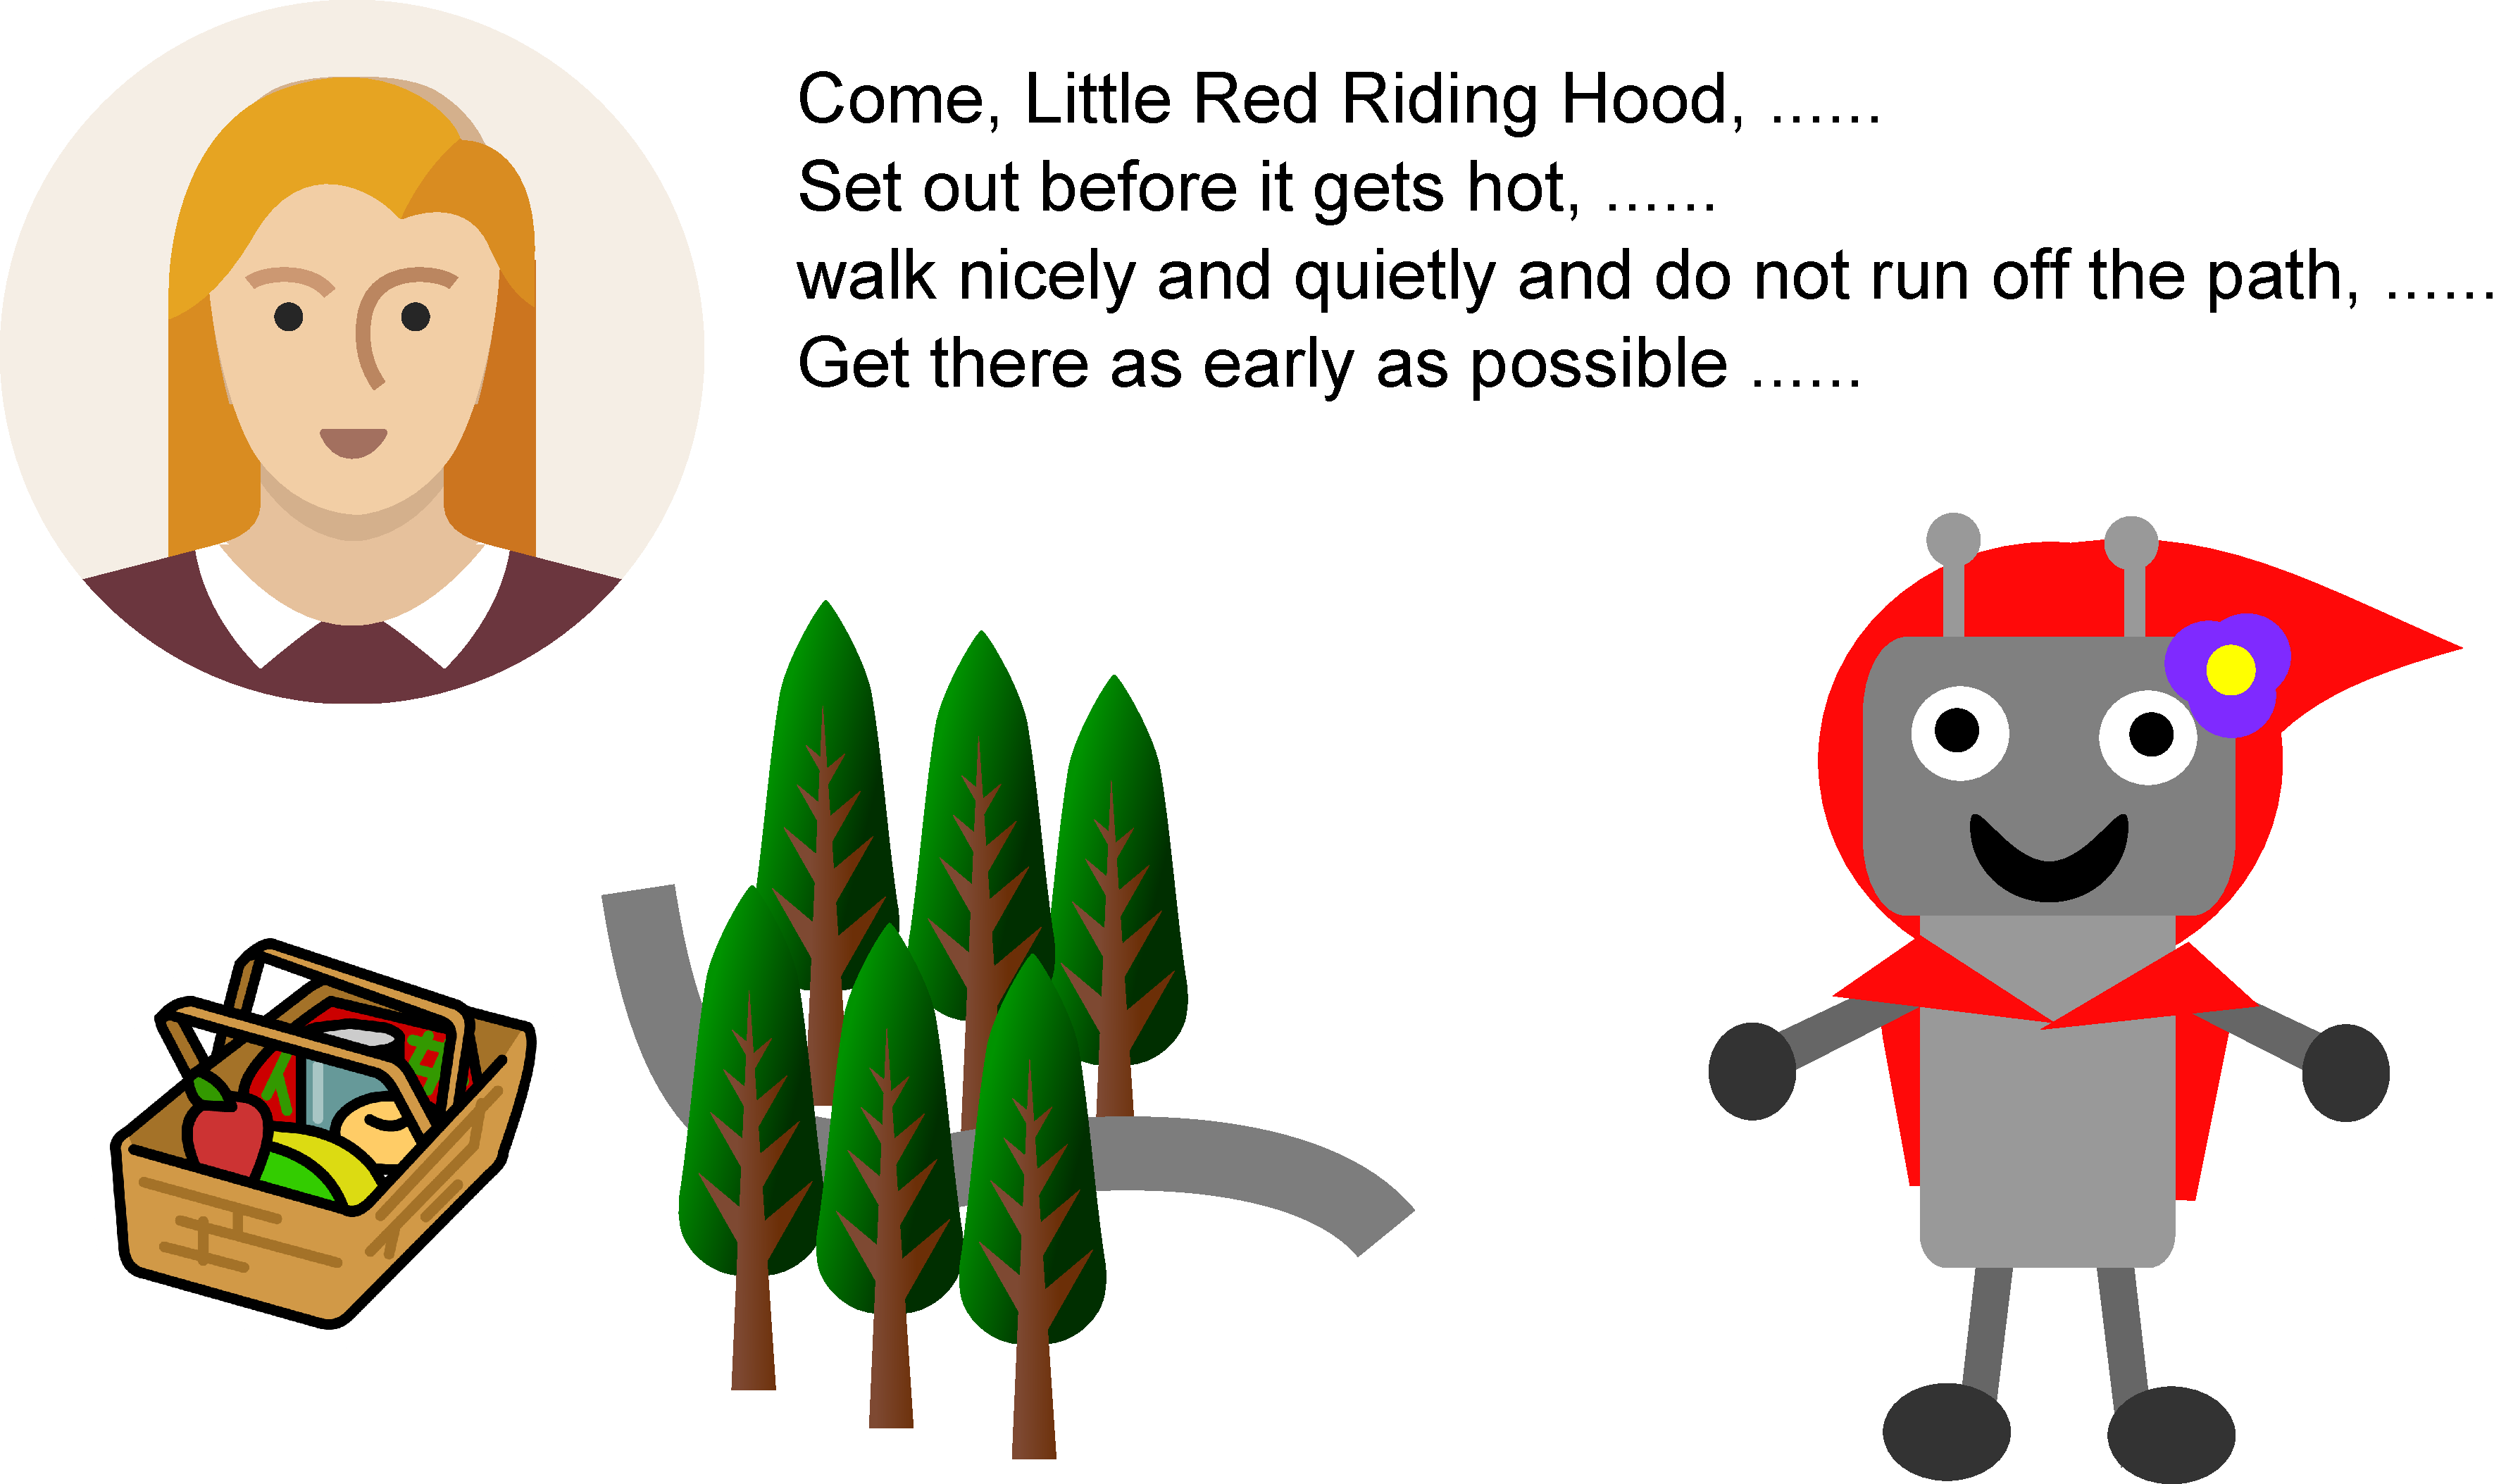
\includegraphics[width=\linewidth]{figure/task_assign}
		%\caption{}
		\label{fig:task_assign}
	\end{figure}
\end{frame}

\begin{frame}{The need of multi-objective}{Introduction}
Objectives
\begin{itemize}
\item \textbf{walk nicely}
\item \textbf{walk quietly}
\item \textbf{as early as possible}
\end{itemize}
Constraints
\begin{itemize}
\item  \textbf{set out before it gets hot}
\item \textbf{do not run off the path}
\end{itemize}
\end{frame}

\begin{frame}{The difficulty in multi-objective}{Introduction}
The problems in modeling human intent
\begin{itemize}
\item incomparability in objectives
\item conflict in objectives
\item hardness in weighing the objectives
\item vagueness in importance selection
\end{itemize}
\begin{figure}
	\centering
	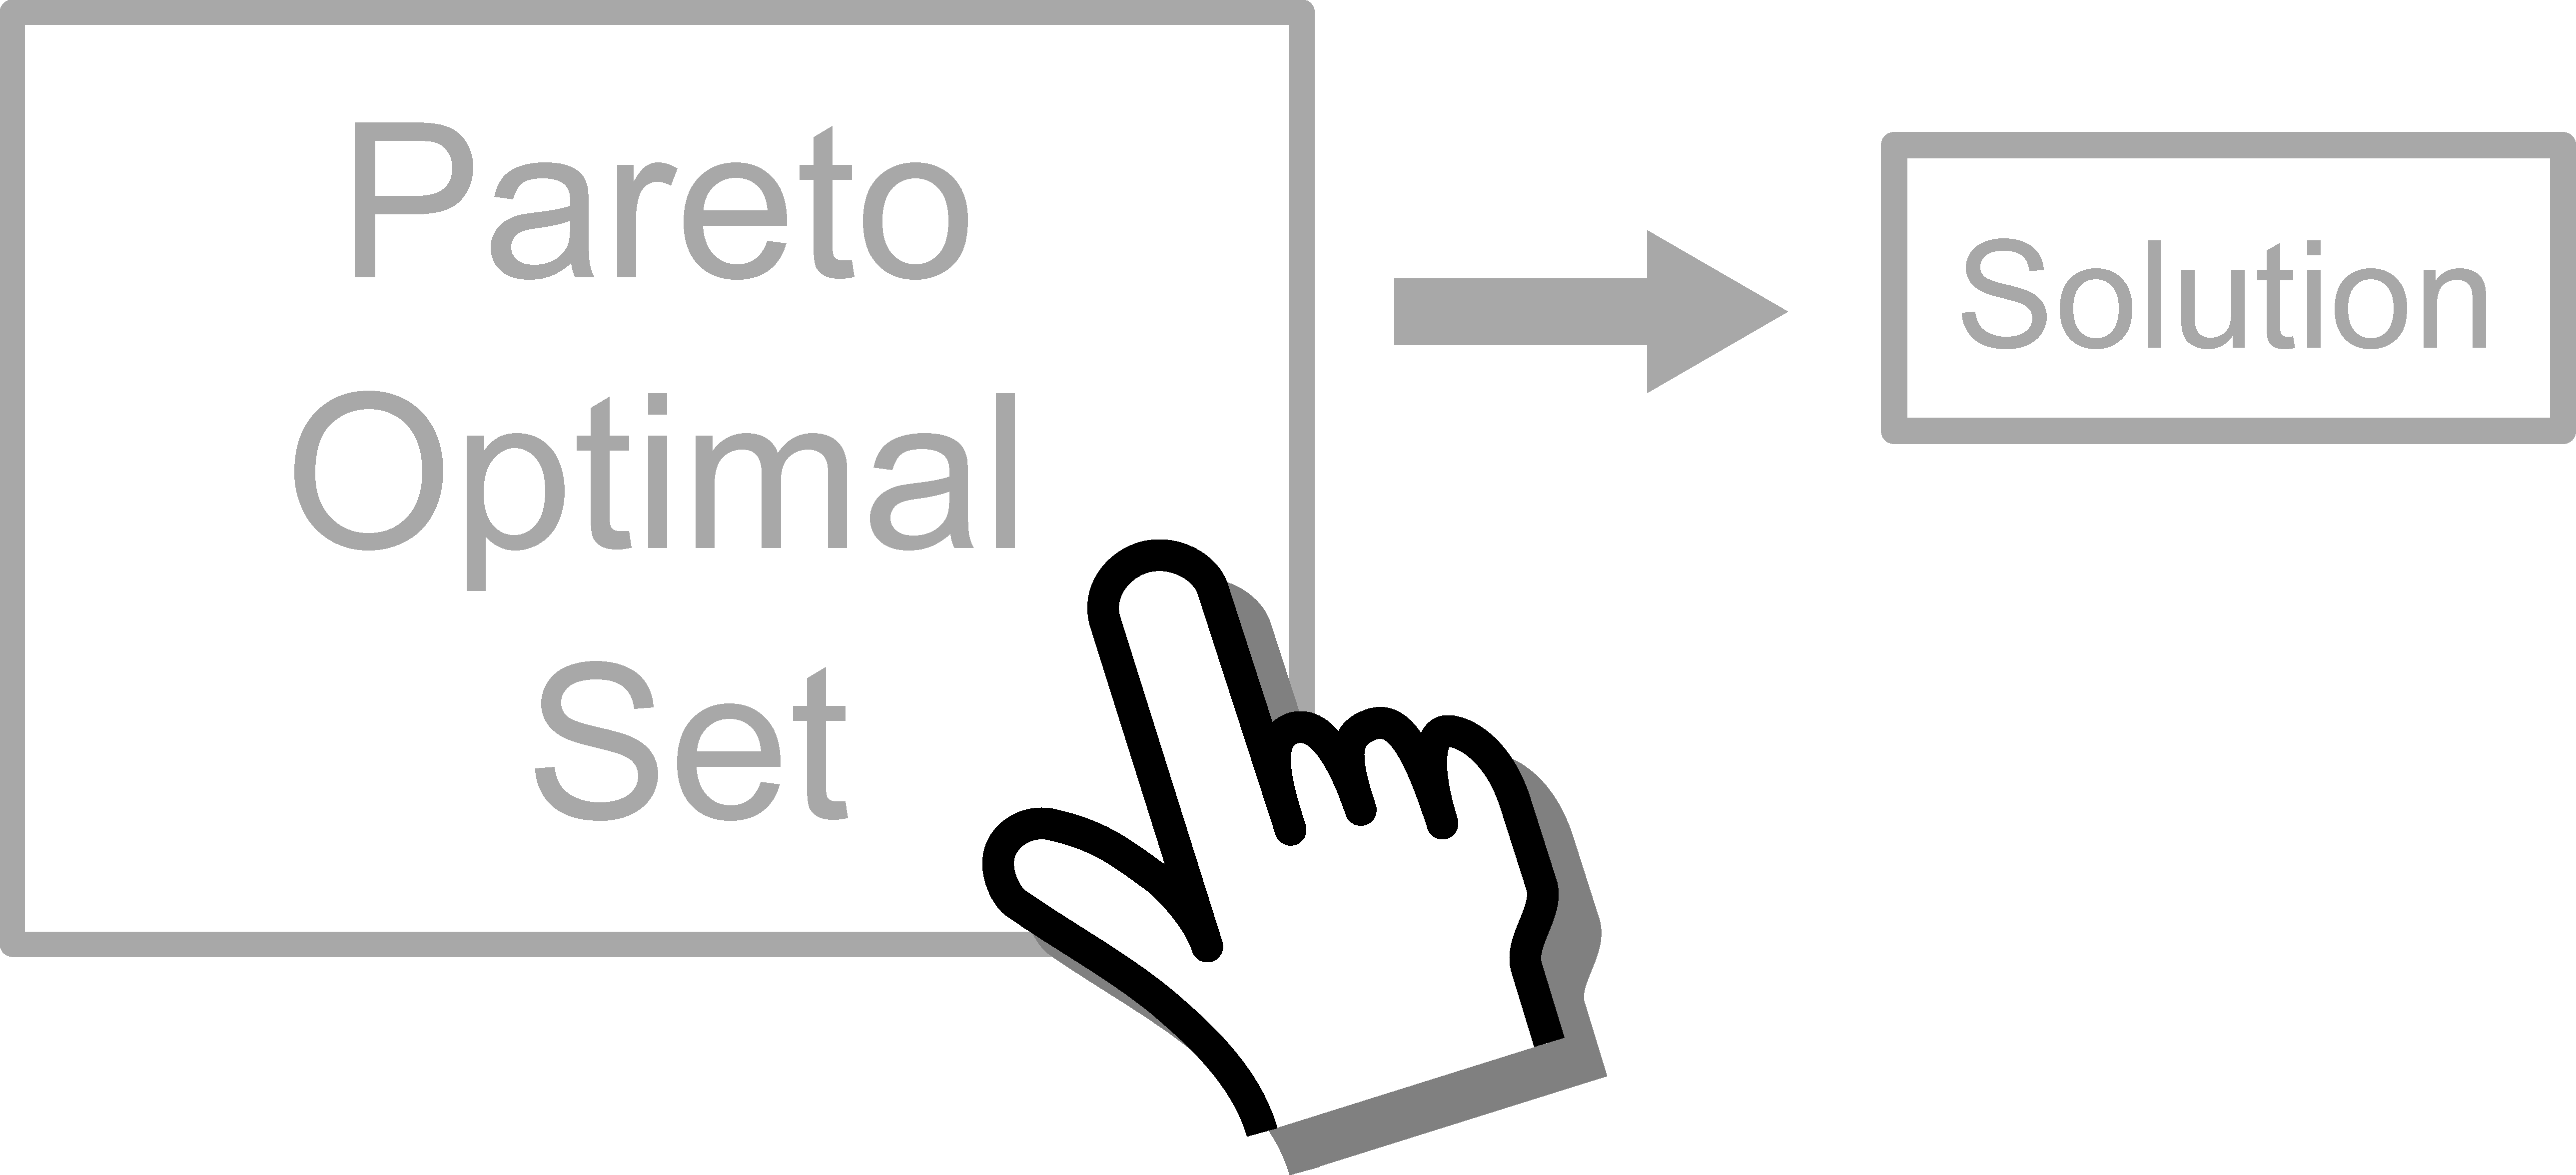
\includegraphics[width=0.6\linewidth]{figure/human_interactive_moo}
	%\caption{}
	\label{fig:human_interactive_moo}
\end{figure}
\end{frame}

\begin{frame}{Pareto Optimal}{Introduction}
%What is Pareto optimal
\begin{columns}
\column{0.5\textwidth}
	\begin{figure}
		\centering
		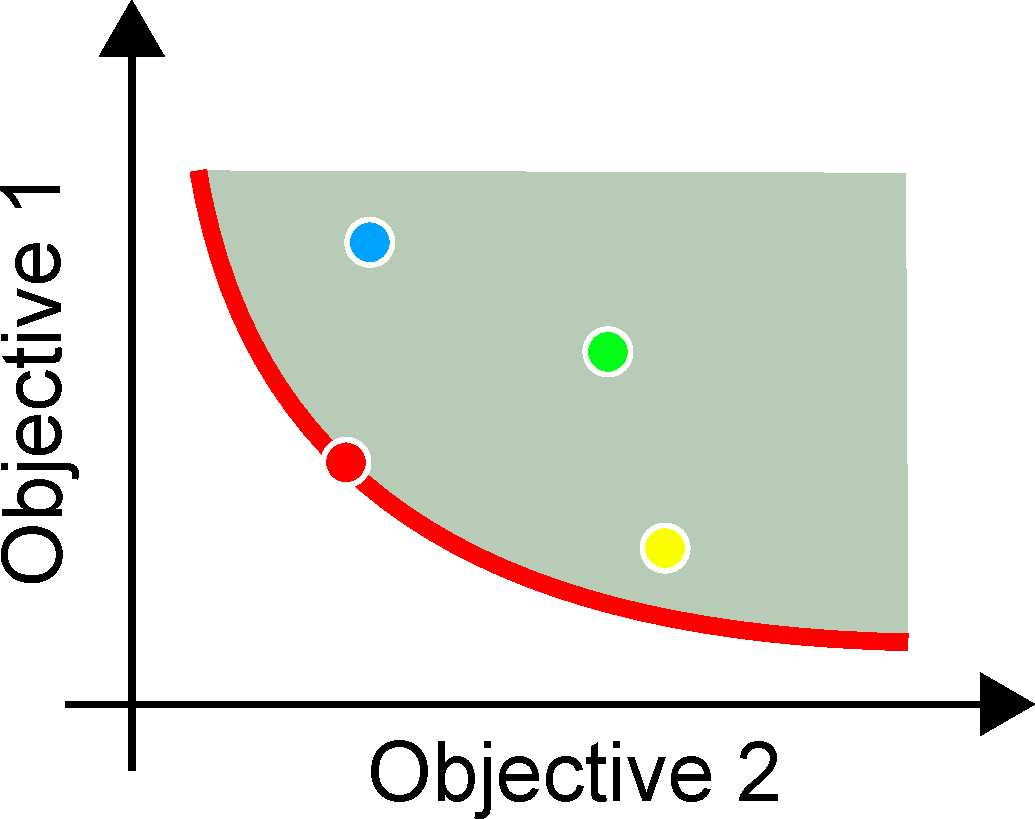
\includegraphics[width=\linewidth]{figure/pareto_optimal}
		%\caption{}
		\label{fig:pareot_optimal}
	\end{figure}
\column{0.5\textwidth}
\begin{minipage}{\textwidth}
\begin{itemize}
\item Non-dominance
\item 
\end{itemize}
\end{minipage}
\end{columns}
\end{frame}

\begin{frame}{Hardness in finding Pareto optimality}{Introduction}

\end{frame}